\documentclass{article}

\usepackage[utf8]{inputenc}

\usepackage{graphicx}

\usepackage{caption}

\usepackage{listings}

\usepackage{minted}

\usepackage{lastpage}

\captionsetup[figure]{name={caption}}

\usepackage[export]{adjustbox} %center

% pakiety do języka polskiego
\usepackage[T1]{fontenc}
\usepackage[polish]{babel}
\usepackage[utf8]{inputenc}

\usepackage{indentfirst} % wcięcia

\title {Specyfikacja Implementacyjna Projektu \\ ,,Game of tanks''} 

\author{Andrzej Czechowski, Bartosz Zakrzewski}

\date{Data utworzenia: 03.04.2020 \\ Data ostatniej modyfikacji: 19.04.2020}

% Nagłówki na każdej stronie
\usepackage{fancyhdr}
\pagestyle{fancy}
\fancyhf{}
\rhead{Andrzej Czechowski, Bartosz Zakrzewski}
\lhead{Specyfikacja Impl. ,,Game of tanks''}
\rfoot{Strona \thepage \hspace{1pt} z \pageref{LastPage}}

\begin{document}
\maketitle
\thispagestyle{empty}

\clearpage

\section{Cel projektu} 

Celem projektu jest stworzenie gry zręcznościowej za pomocą języka programowania Java. Gra otworzy się w okienku z elemetami graficznymi. Będzie w niej dwóch graczy, którzy będą mogli sterować własnymi czołgami i strzelać za pomocą klawiszy na klawiaturze. Gra będzie sprawdzać czy warunki wygranej zostaną spełnione i oznajmiać zwycięzcę. Użytkownik będzie mógł podać plik wejściowy, który zmieni wartości liczb opisujących zasady gry oraz zobaczyć stan planszy (jako plik PNG) po ukończeniu gry.

\section{Środowiska pracy}

Będziemy używać programu IntelliJ IDEA wersji 2020.1 jako domyślnego środowiska programistycznego (IDE):\\

\begin{figure} [hbt!]
   
\includegraphics[width=5cm, center]{img/Intellij.JPG}
   \captionof{figure}{IntelliJ 2020.1}
\end{figure}\\

Najnowsza wersja JDK (Java Development Kit) na dzień 15.04.2020 to 14 i jej będziemy używać.
\begin{figure} [hbt!]
    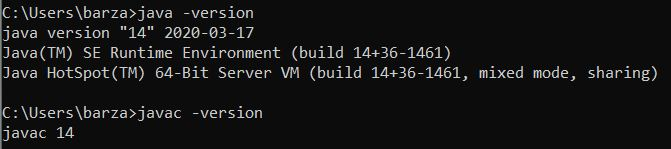
\includegraphics[width=13cm, center]{img/zb_java_windows.JPG}
    \captionof{figure}{Wersja javy}
\end{figure}\\

\clearpage

\begin{figure} [hbt!]
    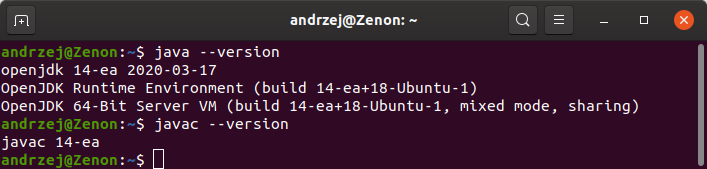
\includegraphics[width=13cm, center]{img/ac_java_ubuntu.png}
    \captionof{figure}{Wersja javy}
\end{figure}\\

Praca będzie odbywać się na systemach operacyjnych Linux (Ubuntu) oraz Windows (10).

\begin{figure} [hbt!]
    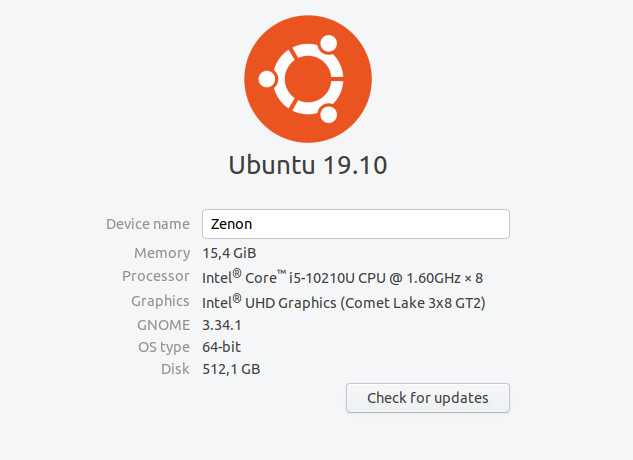
\includegraphics[width= 8cm, center]{img/Wersja_SO.jpg}
    \captionof{figure}{Środowisko pracy Andrzeja Czechowskiego}
\end{figure}\\
\begin{figure} [hbt!]
    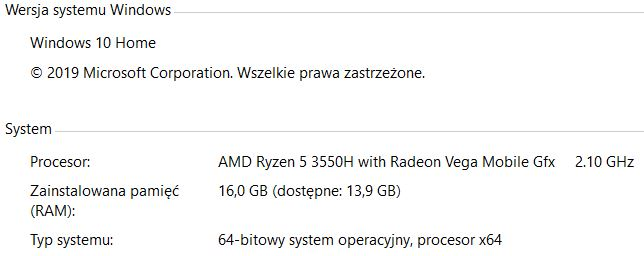
\includegraphics[width= 8cm, center]{img/zb_Windows10.JPG}
    \captionof{figure}{Środowisko pracy Bartosza Zakrzewskiego}
\end{figure}
\clearpage

\section{Zasady komunikacji}

\par Stworzyliśmy oddzielną grupę na messengerze, gdzie będziemy komunikować postępy prac, zamieszczać screeny, zdjęcia i robocze dokumenty.
\par W kodzie będziemy pisać po polsku komentarze robocze - o postępach, rzeczach do zrobienia, błędach itp. 
\par Dodatkowo przynajmniej raz w tygodniu będzie mieli wideokonferencję, aby omówić postępy pracy oraz podzielić się zadaniami.

\section{Zasady pracy}

\subsection{Używanie systemu kontroli wersji}
Kolejne wersje programu będą umieszczane i zapisywane za pomocą systemu kontroli wersji git. Kod oraz dokumentacja będzie trafiać na repozytorium o nazwie ,,Git\_proj'' w folderze Game\_of\_tanks. \\

\par Zasady tworzenia i działania na gałęziach:
\begin{itemize}
    \item Na każdej gałęzi dodajemy funkcjonalność, która po przetestowaniu trafia na mastera.
    \item Na gałąź master trafia tylko kod przetestowany i dający się skompilować.
    \item Gałęzie będą numerowane i ich nazwy będą po angielsku, zgodnie z schematem n\_NameBranch, gdzie n jest numerem gałęzi.
    \item Nazwa gałęzi będzie starać się opisywać dodaną funkcjonalność.
    
\end{itemize}

\par Zasady tworzenia komentarzy przy commitach:
\begin{itemize}
    \item Komentarz ma opisywać dodaną funkcjonalność, (opcjonalnie) możliwe rzeczy do poprawy oraz błędy.
    \item Komentarze piszemy po polsku.
\end{itemize}
Przykładowy commit: ,,tworzenie losowych komórek, nieefektywne tworzenie dzieci''. \\

\par Tagi:
\begin{itemize}
    %\item Jako, że na mastera trafia kod przetestowany, to nie będziemy oznaczać wersji stabilnych.
    \item Wersja, którą będziemy chcieli oddać jako wersję finalną oznaczymy tagiem FINAL (lub podobnym - określonym przez osobę sprawdzającą projekt np. FINAL\_RELEASE\_1).
\end{itemize}

\par Kod przed commitem ma być sformatowany (za pomocą opcji w Intellij'u).

\subsection{Zasady nazewnictwa} 

\par Nazewnictwo w programie będzie w języku angielskim oraz zgodne z notacją Javy (,,camelCase'' oraz ,,UpperCamelCase'')
np. 
\begin{itemize}
    \item GameObject, 
    \item gameState,
    \item createRandomCell().
\end{itemize}

Nazwy folderów, dokumentów czy pakietów mogą być oddzielone \\ znakiem ,,\_''. Mogą być one także po polsku.
np. 
\begin{itemize}
    \item game (pakiet)
    \item Specifications (folder)
    \item Specyfikacja\_Implementacyjna.pdf (dokument)
    \item Implementation\_Specification.pdf (dokument)
\end{itemize}

Nazwy funkcji testujących również mogą (ale nie muszą) zawierać znak ,,\_''.
np.
\begin{itemize}
    \item wrongFormattedVariable\_makeItDefault()
    \item exceedMaxPointsToWin()
    \item collisionWithCell\_shouldDestroyBullet()
\end{itemize}

\par Komentarze w kodzie ,,roboczym'' (wersje dla członków zespołu) (aby łatwiej było się komunikować oraz mieć rozpisane co trzeba poprawić) mogą być po polsku.
\par Jeżeli kod będzie zawierał komentarze dla osoby z poza zespołu (np. wyjaśniające wartość nieintuicyjnej zmiennej) będą po angielsku.

\clearpage

\section{Struktura programu} 

\subsection{Diagram klas}

\begin{figure} [hbt!]
   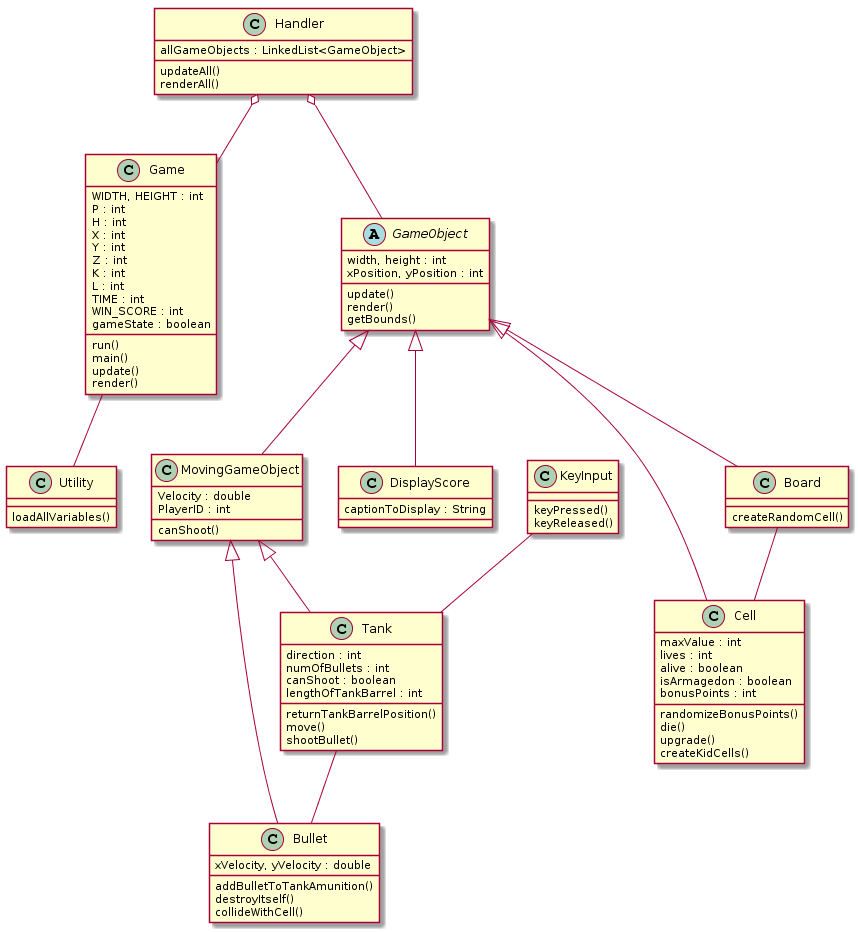
\includegraphics[width=14cm, center]{img/diagramKLAS_1.png}
   \captionof{figure}{Diagram klas}
\end{figure}

% opis diagramu  znaczenie i działanie klas, pola, metody
A - klasa abstrakcyjna, C - klasa
\clearpage

\subsection{Importy}

Potencjalne importy: (tutaj też korzystamy z: \\ 
https://www.youtube.com/watch?v=JrSjwQbTldg, marcusman.com)
\begin{itemize}
    \item import java.awt.Graphics (renderowanie)
    \item import java.awt.Rectangle (do getBounds() - obsługa kolizji)
    \item import java.awt.Canvas (pozwala na rysowanie)
    \item import java.awt.image.BufferStrategy (mechanizm ,,ładowania'' i wyświetlania grafiki)
    \item import java.util.LinkedList
    \item import java.awt.event.KeyListener
    \item import java.awt.event.KeyEvent
    \item import javax.swing.JFrame
    \item import java.awt.Color;
\end{itemize}

Pobieranie i wyświetlanie obrazów:
\begin{itemize}
    \item import java.awt.image.BufferedImage
    \item import java.io.File
    \item import java.io.IOException
    \item import javax.imageio.ImageIO
    \item import javax.swing.JPanel
\end{itemize}

Pozostała importy to wyświetlenie tekstu (numeru - wartości komórki) oraz inne, które będziemy poznawać podczas implementacji.

Podczas implementacji ustalimy czy potrzebujemy kilku pakietów, na początku wszystkie klasy umieścimy w jednym o nazwie game.

% pakiety
% foldery
Folder images będzie przechowywał obrazki, a folder data będzie plik konfiguracyjny.

\clearpage

\section{Kolejność działania}
Prace podzielimy na dwa sprinty.\\
Pierwszy będzie trwał do Proof of concept (13.05.2020):
\begin{enumerate}
    \item Pętla odtwarzająca program (funkcja run()) oraz okienko za pomocą JFrame).
    \item Dodawanie obiektów (GameObject) do okienka aplikacji.
    \item Plansza składająca się z losowych komórek (klasa Board).
    \item Rodzenie się komórek-dzieci (klasa Cell).
    \item Ruch pocisku (przy ustalonym punkcie początkowym i kącie strzelania).
    \item Kolizja pocisku z komórką.
    \item Dodanie schematu czołgu, w którym można poruszać lufą.
    \item Strzelanie pocisków przy możliwości zmiany kąta. 
    \item Zdobywanie punktów.
    \item Tworzenie pliku JAR oraz uruchamianie programu.
\end{enumerate}

Drugi sprint do 03.06.2020:
\begin{enumerate}
    \item Dodanie drugiego gracza.
    \item Tworzenie klasy DisplayScore (okienka timer i score).
    \item Wczytywanie z pliku wejściowego danych konfiguracyjnych. 
    \item Obsługa punktów spadkowych.
    \item Zmniejszanie się rozmiaru komórek.
    \item Inne możliwości wygrywania.
    \item Tworzenie pliku wyjściowego PNG.
\end{enumerate}

Zakres prac czy kolejność wykonywania zadań może być lekko zmieniona podczas implementacji. \\
Po pierwszym sprincie będziemy chcieli osiągnąć grę, która będzie działać, ale nie będzie musiała spełniać wszystkich funkcjonalności. \\ Natomiast drugi sprint będzie trwał do terminu oddania projektu.

\clearpage

\section{Istotne Algorytmy w programie}

\subsection{Skalowanie rozmiarów obiektów}

Użytkownik ma mieć możliwość zmiany rozmiarów planszy (tutaj zamiast planszy z komórkami - Board mamy jednak na myśli okienko JFrame z całą grą (jego WIDTH oraz HEIGHT)). \\
Aby móc przeskalować inne elementy gry (aby ich rozmiar był zgodny z rozmiarem aplikacji) utworzymy dwie zmienne: \\

\begin{itemize}
    \item $p_w = \frac{WIDTH}{defaultWidth}$ 
    \item $p_h = \frac{HEIGHT}{defaultHeight}$
\end{itemize}
gdzie: \\
WIDTH, HEIGHT - zmienne wejściowe, \\
defaultWidth, defaultHeight - domyślny rozmiar okienka JFrame. \\

Następnie wysokość i szerokość każdego obiektu będzie skalowana zgodnie ze schematem:

w, h - domyślne rozmiary obiektu,

$ w \cdot p_w$, $h \cdot p_h $ - rozmiary obiektu po przeskalowaniu. 

\subsection {Obliczanie aktualnego położenia posicku}

Pocisk będę miał własną prędkość (V) (która będzie się zwiększała podczas gry).
Aby pocisk mógł się poruszać po planszy w zależności od miejsca wystrzelenia (kąta lufy) nadamy mu dwie prędkości składowe Vx i Vy.

Algorytm zmiany położenia pocisku: \\ \\
V - prędkość wystrzelonego pocisku wyrażona w ilościach pikseli na t \\
t - czas odświeżania (1/60 s) (nadamy grze 60 FPS'ów (60 klatek na sekundę)) \\
$\alpha$ - kat wystrzelonego pocisku  \\
x, y - polozenie pocisku przed odświeżeniem\\
$x + V\cos(\alpha)\cdot t$, $y + V\sin(\alpha)\cdot t$ - położenie pocisku po odświeżeniu \\

\clearpage

\subsection {Funkcja run() i jej opis}

\begin{minted} {Java}
    private boolean gameState = true;

    public void run() {

        long lastTime = System.nanoTime();
        double nanoSecondFpsConversion = 1000000000.0 / 60;
        double deltaTime = 0;

        while (gameState) {
            long now = System.nanoTime();

            deltaTime += (now - lastTime) / nanoSecondFpsConversion;
            while (deltaTime >= 1) {
                update();
                deltaTime--;
            }

            render();
            lastTime = now;
        }
    }

    public static void main(String[] args) {
        Game game = new Game();
        Thread gameThread = new Thread(game);
        gameThread.start();
    }

\end{minted}

Klasa Game implementuje interfejs Runnable. Następnie wątek gameThread, a wraz z nim funkcja run() będzie zajmować się obsługą naszej gry. Ustawiliśmy nasze zmienne tak, aby co 1/60 sekundy (czyli 60 klatek/odświeżeń/update'ów na sekundę) odświeżał się stan gry. Sprawi to, że niezależnie na jakim komputerze, gra będzie ,,chodziła'' tak samo szybko.

\clearpage

\subsection{Pozostałe algorytmy}

Inne istotne algorytmy będę musiały zostać opracowane podczas pisania kodu (np. podczas wideo-rozmów). 
Są to np. 
\begin{itemize}
    \item Częstotliwość i prawdopodobieństwo punktów spadkowych.
    \item Działanie równoległe programu (podział na wątki).
    \item Obsługa wyjątków (Exceptions).
    \item Log programu (gdzie wypisujemy komunikaty - błędy).
    \item Animacje (poruszanie lufy itp.).
\end{itemize}

Również możemy napotkać ograniczenia i rzeczy, których nie będziemy potrafili napisać. Będzie musiało to zostać udokumentowane w Proof of Concept lub w Sprawozdaniu Końcowym.

\section{Testowanie}
Testy jednostkowe będzie pisać z wykorzystaniem biblioteki AssertJ.
Planujemy robić testy na poszczególnych gałęziach a dopiero następnie mergować kod na mastera.

\section{Źródła}
\begin{itemize}
    \item Tobiasz Siemiński - opis specyfikacji implementacyjnej: \\ https://sortris.blogspot.com/2010/08/jak-napisac-specyfikacje.html?m=1
    
    \item Ten dokument został utworzony w LaTeX'ie za pomocą strony \\ https://www.overleaf.com
    
    \item Jest to drugi z kolei dokument dotyczący projektu ,,Game\_of\_tanks''

    \item Początkowa struktura gry, pętla run() oraz diagram klas na podstawie: \\
    https://marcusman.com/ oraz \\
    Java Programming: Let's Build a Game by RealTutsGML \\ 
    (https://www.youtube.com/watch?v=1gir2R7G9ws)
    
    \item Diagramy klas: \\
    https://www.p-programowanie.pl/uml/diagramy-klas-uml/ \\
    http://zasoby.open.agh.edu.pl/~09sbfraczek/diagram-klas\%2C1\%2C11.html
    
    \item Diagram klas wykonany za pomocą \\ https://plantuml.com/class-diagram
    
    \item Importy do wyświetlania obrazków: \\ https://javastart.pl/baza-wiedzy/grafika\_awt\_swing/pobieranie-i-wyswietlanie-obrazow
    
\end{itemize}

\end{document}
